\documentclass{article}


% if you need to pass options to natbib, use, e.g.:
%     \PassOptionsToPackage{numbers, compress}{natbib}
% before loading neurips_2025

\PassOptionsToPackage{numbers, compress}{natbib}

% ready for submission
\usepackage{neurips_2025}


\bibliographystyle{abbrvnat}

\usepackage[pdftex]{graphicx}
\usepackage{amsmath}
% to compile a preprint version, e.g., for submission to arXiv, add add the
% [preprint] option:
%\usepackage[preprint]{neurips_2025}


% to compile a camera-ready version, add the [final] option, e.g.:
%     \usepackage[final]{neurips_2025}


% to avoid loading the natbib package, add option nonatbib:
%    \usepackage[nonatbib]{neurips_2025}


\usepackage[utf8]{inputenc} % allow utf-8 input
\usepackage[T1]{fontenc}    % use 8-bit T1 fonts
\usepackage{hyperref}       % hyperlinks
\usepackage{url}            % simple URL typesetting
\usepackage{booktabs}       % professional-quality tables
\usepackage{amsfonts}       % blackboard math symbols
\usepackage{nicefrac}       % compact symbols for 1/2, etc.
\usepackage{microtype}      % microtypography
\usepackage{xcolor}         % colors

\newcommand\reynotes[1]{\textcolor{purple}{#1}}

%\title{SmokeViz: Using Pseudo-Labels to Develop a Human-Labeled Deep Learning Dataset of Wildfire Smoke Plumes in Satellite Imagery}
\title{SmokeViz: A Large-Scale Satellite Dataset for Wildfire Smoke Detection and Segmentation}


% The \author macro works with any number of authors. There are two commands
% used to separate the names and addresses of multiple authors: \And and \AND.
%
% Using \And between authors leaves it to LaTeX to determine where to break the
% lines. Using \AND forces a line break at that point. So, if LaTeX puts 3 of 4
% authors names on the first line, and the last on the second line, try using
% \AND instead of \And before the third author name.


\author{%
  Rey Koki\\%\thanks{rey.koki@colorado.edu} \\
  Department of Computer Science\\
  University of Colorado Boulder\\
  Boulder, Colorado 80303\\
  \texttt{rey.koki@colorado.edu} \\
  % examples of more authors
  % \And
  % Coauthor \\
  % Affiliation \\
  % Address \\
  % \texttt{email} \\
  % \AND
  % Coauthor \\
  % Affiliation \\
  % Address \\
  % \texttt{email} \\
  % \And
  % Coauthor \\
  % Affiliation \\
  % Address \\
  % \texttt{email} \\
  % \And
  % Coauthor \\
  % Affiliation \\
  % Address \\
  % \texttt{email} \\
}


\begin{document}


\maketitle


\begin{abstract}
    The global rise in wildfire frequency and intensity over the past decade underscores the need for improved fire monitoring techniques. To advance deep learning research on wildfire detection and its associated human health impacts, we introduce \textbf{SmokeViz}, a large-scale machine learning dataset of smoke plumes in satellite imagery. The dataset is derived from expert annotations created by smoke analysts at the National Oceanic and Atmospheric Administration, which provide coarse temporal and spatial approximations of smoke presence. To enhance annotation precision, we propose \textbf{pseudo-label dimension reduction (PLDR)}, a generalizable method that applies pseudo-labeling to refine datasets with mismatching temporal and/or spatial resolutions. Unlike typical pseudo-labeling applications that aim to increase the number of labeled samples, PLDR maintains the original labels but increases the dataset quality by solving for intermediary pseudo-labels (IPLs) that align each annotation to the most representative input data. For SmokeViz, a parent model produces IPLs to identify the single satellite image within each annotations time window that best corresponds with the smoke plume. This refinement process produces a succinct and relevant deep learning dataset consisting of over 180,000 manual annotations. The SmokeViz dataset is expected to be a valuable resource to develop further wildfire-related machine learning models and is publicly available at \url{https://noaa-gsl-experimental-pds.s3.amazonaws.com/index.html#SmokeViz/}.
\end{abstract}


\section{Introduction}

Due in part to public policy, average fine particulate matter (PM\textsubscript{2.5}) levels in the United States have declined over recent decades \cite{clean_air_act}. However, from 2010 to 2020, the contribution of wildfire smoke to PM\textsubscript{2.5} concentrations more than doubled, accounting for up to half of total PM\textsubscript{2.5} exposure in Western U.S. \cite{smoke_PM}. This is particularly concerning, as ambient PM\textsubscript{2.5} is a leading environmental risk factor for adverse health outcomes and premature mortality \cite{smoke_mortality}. These trends/risks highlight the urgent need for scalable and timely smoke monitoring systems to mitigate public health risks.

Satellite imagery offers the spatial coverage and temporal frequency needed for large-scale smoke monitoring. In comparison to polar-orbiting satellites like Suomi or Sentinel, geostationary satellites such as the GOES series \cite{goes} are especially well-suited to this task, providing persistent observation over fixed regions—essential for capturing the dynamic behavior of wildfire smoke plumes. The high temporal resolution and wide coverage of GOES imagery enable real-time tracking of smoke concentration and movement, supporting air quality assessments and early warning systems.

Even with the advances in remote sensing, existing deep learning satellite datasets for wildfire smoke detection face several limitations. They are often small in scale, restricted to specific regions or events, and focus on scene-level classification rather than pixel-level segmentation. Most do not differentiate between smoke density levels, are not publicly available, and lack standardized benchmarks for semantic segmentation. While NOAA’s Hazard Mapping System (HMS) provides a large-scale, expert-labeled dataset, its annotations span multi-hour time windows that vary in duration. This creates a temporal mismatch between the labels and individual satellite frames, complicating their direct use for supervised learning.

To address these challenges, we introduce \textbf{SmokeViz}, a large-scale satellite dataset for semantic segmentation of wildfire smoke plumes. SmokeViz includes over 180,000 annotated samples derived from GOES-East and GOES-West imagery, aligned with HMS analyst annotations. To resolve the temporal ambiguity in the original labels, we propose a semi-supervised method called \textbf{pseudo-label dimension reduction (PLDR)}, which uses intermediary pseudo-labels to select the satellite image that best matches each smoke annotation. The resulting dataset provides one-to-one image-to-label pairs with ordinal smoke density masks, suitable for supervised deep learning.

\textbf{SmokeViz} serves as a benchmark for wildfire smoke segmentation and as a resource for the broader machine learning community working with geospatial, temporal, and remote sensing data. It supports new directions in ordinal segmentation, semi-supervised learning with temporal uncertainty, and pretraining for Earth observation tasks involving dynamic atmospheric phenomena.

The contributions presented in this paper include \textbf{SmokeViz}, the largest satellite-based dataset for wildfire smoke segmentation, with over 180,000 samples from GOES imagery, our proposed \textbf{PLDR}, a physics-guided semi-supervised method for aligning coarse human annotations with temporally optimal satellite imagery and benchmark segmentation baselines with standardized training splits to support reproducibility and future studies.

\section{Related Work}

\subsection{Smoke Detection and Labeling Methods}

Multi-channel thresholding remains a widely used method for distinguishing smoke from similar atmospheric signatures such as dust or clouds using channel-specific radiance values \cite{threshold}. These thresholds are typically derived from labeled historical data and are fine-tuned to specific regions and fuel types, limiting their generalizablity \cite{thresh_geog}. In contrast, the SmokeViz dataset spans a wide range of biogeographies across North America and can serve as a source of refined analyst-labeled examples for developing more generalizable thresholding techniques.

Large parameterized numerical models are used for forecasting smoke dispersion, but not for smoke detection itself. Systems such as HRRR-Smoke and RRFS \cite{hrrr, rrfs} rely on computationally intensive forecasts requiring nearly 200 dynamic meteorological inputs. A key limitation of these models is the absence of a real-time smoke analysis product for data assimilation, resulting in delayed model spin-up and compounded forecast errors. Model predictions from SmokeViz could help fill this gap, offering a real-time, satellite-driven alternative to support data assimilation for operational smoke dispersion forecasting.

Manual smoke labeling is performed by trained analysts through visual inspection of satellite imagery. NOAA’s Hazard Mapping System (HMS) provides a analyst-labeled wildfire smoke dataset \cite{hms, hms_val}. HMS analysts examine GOES imagery sequences to track smoke plume movement and annotate the approximate spatial extent and qualitative density of smoke (light, medium, heavy), as illustrated in Figure \ref{densities}. Annotations are issued on a rolling basis and span time windows ranging from instantaneous to over 20 hours \cite{hms_web}. While HMS provides high-quality expert annotations, its operational format introduces challenges for supervised learning: annotations are temporally coarse, vary in length, and lack one-to-one correspondence with satellite frames. SmokeViz refines HMS annotations into temporally resolved, frame-aligned labels, enabling real-time, continuous predictions of smoke extent and density.

\begin{figure}[!htb]
    \centering
    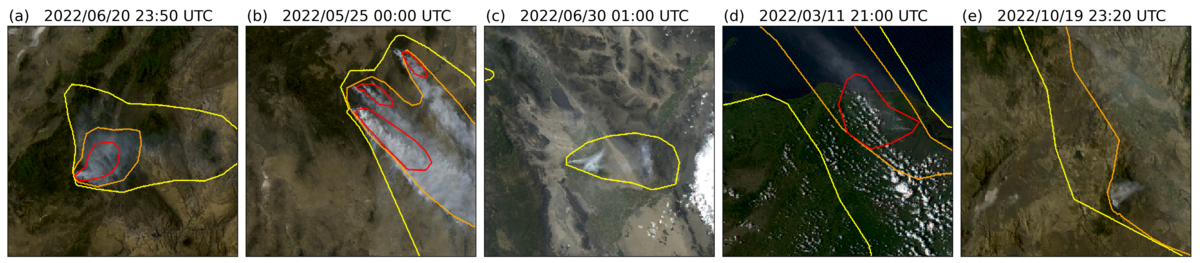
\includegraphics[width=\linewidth]{figures/variations_small.png}\label{densities}
    \caption{HMS smoke annotations overlaid on GOES imagery. Yellow, orange, and red contours indicate light, medium, and heavy smoke density, respectively. (a) and (b) show canonical smoke plumes; (c)–(e) illustrate density label variation across scenes.}
\end{figure}

\subsection{Deep Learning Datasets and Models for Wildfire Smoke}

Recent efforts have applied deep learning to wildfire smoke detection using a variety of satellite sources and label strategies. SmokeNet \cite{smokenet} employs a convolutional neural network (CNN) to classify MODIS image scenes as containing smoke or not, using student-provided labels. SatlasPretrain \cite{satlas} includes a small set of Sentinel-2 images labeled for smoke as part of a larger multi-label pretraining dataset. While scene classification methods can provide wildfire detection information, they do not capture spatial characteristics of smoke plumes that segmentation would be more appropiate to capture.

Several datasets have been developed for smoke segmentation, but they are limited in scope. Wen et al.\ \cite{smoke_goes} trained a CNN on GOES-East imagery over California and Nevada using HMS annotations from the 2018 wildfire season. Larsen et al.\ \cite{larsen} used Himawari-8 data to detect smoke at the pixel level for a single fire event, using a threshold-based algorithm as ground truth. Table \ref{studies} compares these datasets in terms of scale, source, and labeling. SmokeViz stands out by offering over 180,000 samples with analyst-generated, frame-aligned labels covering multiple fire seasons, regions, and biogeographies. Not only do we use geostationary satellites with persistent observations, but we choose either GOES-East or GOES-West based on which satellite has optimal observational conditions of the event. It is, to our knowledge, the largest and most diverse dataset for smoke plume segmentation.


\begin{table*}[h]
    \caption{Comparison of satellite smoke plume datasets, detailing the number of smoke plume samples, satellite source (polar orbiting (P) or geostationary (G)), number of spectral bands, labeling method, classification type - scene classification (SC) or semantic segmentation (SS), and public availability.}\label{studies}
    \centering
    \begin{tabular}{ccccrrcrc}
        \toprule
        reference & \verb|#| samples & satellite & \verb|#| bands & label & task & avail.\\
        \midrule
        \cite{smokenet}& 1016 & MODIS (P)& 5 & students & SC & no \\
        \cite{satlas} & 125 & Sentinel-2 (P)& 3 & crowd sourced & SC & yes \\
        \cite{smoke_goes}& 4095 & GOES-East (G)& 5 & HMS analysts & SS & no \\
        \cite{larsen} & 975 & Himiwari-8 (G) & 7 & algorithm& SS & no \\
        %\cite{wang}& 47 & Landsat-8 & 4 & & \\
        SmokeViz  & 183,672 & GOES-East+West (G)& 3 & HMS analysts & SS & yes \\
        \bottomrule
    \end{tabular}
\end{table*}

In addition to its relevance for wildfire applications, SmokeViz contributes a challenging benchmark for general-purpose remote sensing vision tasks. Unlike many existing datasets that avoid cloudy scenes \cite{bigearthnet, crops} or focus on sharply bounded features such as cropland \cite{crops}, infrastructure \cite{polyworld}, or oceanic clouds \cite{cyclone, cloud_texture}, smoke has amorphous, fading boundaries in both space and time. Incorporating smoke segmentation into large-scale pretraining corpora, such as SatlasPretrain \cite{satlas}, could enhance generalizable models for Earth observation.

\subsection{Pseudo-labeling and Semi-Supervised Learning}

Semi-supervised learning techniques such as pseudo-labeling have been widely used to expand training data by leveraging unlabeled samples \cite{pseudo}. Typically, a parent model is trained on labeled data and then used to generate pseudo-labels for an unlabeled dataset, which are in turn used to train subsequent models in an iterative process.

In contrast, we propose a non-iterative variation focused not on data expansion, but dataset data-to-label precision. Our method, \textbf{pseudo-label dimension reduction (PLDR)}, generates intermediary pseudo-labels (IPLs) for each satellite frame within the HMS annotation window. Rather than using these labels for training, we use them to identify the satellite image with the greatest alignment to the analyst annotation. This enables the construction of SmokeViz, a temporally disambiguated, one-to-one image-to-label dataset. The resulting dataset methodically pairs the analyst-generated smoke plume labels with selected GOES imagery, enabling high-resolution, temporally accurate segmentation model training.


Beyond wildfire smoke segmentation, PLDR offers a general framework for aligning coarse or weakly matched datasets. This is particularly useful in domains such as remote sensing, medical imaging, and video analysis, where annotations often span temporal or spatial intervals rather than individual frames. In Earth observation specifically, atmospheric parameters are often combined from disparate sources with inconsistent spatial and temporal resolutions, making it difficult to integrate them into unified training datasets. By using intermediary pseudo-labels to identify the most representative input sample, PLDR transforms many-to-one or one-to-many supervision into clean one-to-one mappings. This enables more precise alignment between data and labels, facilitating integration across heterogeneous sources without requiring additional hand-labeling. As presented, PLDR serves as a practical preprocessing strategy for repurposing historical legacy datasets with temporal ambiguity into precise training resources for modern deep learning models.

\section{Methods}
\subsection{Datasets}

We use imagery from the latest GOES satellites—GOES-16 (East), GOES-17, and GOES-18 (West)—each equipped with the Advanced Baseline Imager (ABI), which captures 16 spectral bands from visible to infrared wavelengths every 10 minutes. We process bands 1-3 using PyTroll \cite{satpy} to generate 1km true-color composites \cite{true_color}, matching the imagery reviewed by HMS analysts. These bands correspond to the shortest wavelengths available on ABI and yield the highest signal-to-noise ratio (SNR).

To approximate the dynamic movement of smoke, HMS analysts annotate plumes using multi-frame satellite animations. These annotations span varying time windows, averaging three hours. Since the HMS annotations are designed to reflect overall plume extent during a time window rather than at any specific moment, smoke boundaries in individual frames may not align well with the annotation (Figure \ref{timelapse}). A naive modeling approach would use all frames within each time window as input, but this introduces non-uniform sequence lengths and significantly increases memory and computational demands and complicates the use of CNN architectures. Instead, we establish a one-to-one mapping by identifying the single satellite frame that best matches each analyst annotation.


\begin{figure}[!htb]
    \centering
    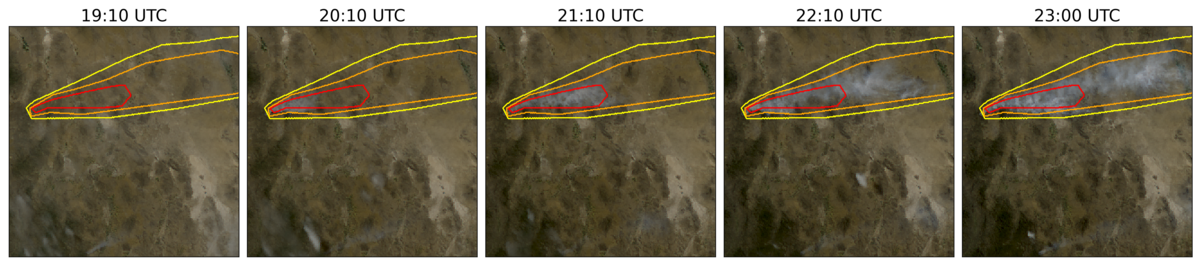
\includegraphics[width=\linewidth]{figures/timelapse_small.png}
    \caption{True color GOES-East imagery from May 5th, 2022, Southeast New Mexico (\(31.38^{\circ}\)N, \(107.87^{\circ}\)W) during the start of the Foster Fire. The red, orange and yellow lines represent the heavy, medium and low density HMS smoke annotations that span 19:10\textendash23:00 UTC.}
    \label{timelapse}
\end{figure}


We select either GOES-East or GOES-West based on the solar zenith angle (SZA) to optimize for forward Mie scattering, which enhances smoke visibility in satellite imagery. Smoke particles (100nm-10\textmu m) scatter light predominantly via Mie scattering when \(\lambda < d\), favoring short wavelengths and forward angles (Figure \ref{mei}). To generate the Mie-derived dataset, we evaluate the available satellite platforms for each annotation time window and choose the satellite (East or West) that is expected to observe the strongest forward scattering geometry based on sun-satellite alignment. This ensures selection of the satellite view with the highest potential smoke SNR if smoke were present. Therefore, we select (1) the satellite expected to yield the strongest Mie forward scattering (Figures \ref{WEST_EAST_bands}(a) vs \ref{WEST_EAST_bands}(b)) and (2) the three shortest wavelength ABI bands (C01-C03: 0.47, 0.64, and 0.865\textmu m) (Figures \ref{WEST_EAST_bands}(c)-\ref{WEST_EAST_bands}(e)).


\begin{figure}[!htb]
    \centering
    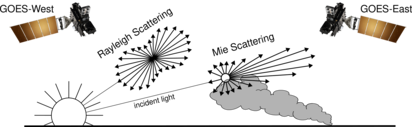
\includegraphics[width=8cm]{figures/mei_small.png}
    \caption{If the particle size is \(<\frac{1}{10}\) the \(\lambda\) of the interacting light, then the primary scattering will be Rayleigh. Mie scattering is the predominant scattering mechanism when the particle size is larger than the \(\lambda\) of light. This schematic demonstrates that when the sun is setting in the West, the Mie scattering will predominately forward scatter towards GOES-East.} \label{mei}
\end{figure}

\begin{figure}[!htb]
    \centering
    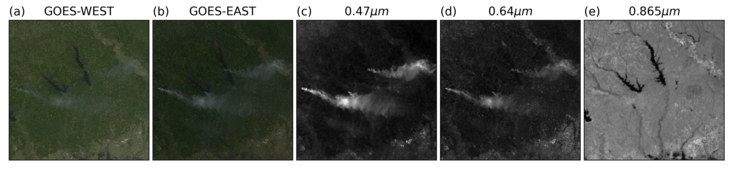
\includegraphics[width=\linewidth]{figures/GOES_WEST_EAST_B_R_V_small.png}
    \caption{True color (a) GOES-WEST and (b) GOES-EAST imagery from March \(23^{rd}\), 2022 centered at (\(31.1^{\circ}\), \(-93.8^{\circ}\)) in Texas, USA taken at 23:20 UTC. The GOES-EAST raw band imagery for (c) blue, (d) red and (e) veggie bands show variations in the SNR for smoke detection in relation to the \(\lambda\) of light being measured.}\label{WEST_EAST_bands}
\end{figure}

\subsubsection{From Full Dataset \(\mathcal{D}\) to Mie-Derived Dataset \(\mathcal{D}_M\)}

Let \(\mathcal{D} = \{\mathcal{X}, \mathcal{Y}\}\) be the original dataset, where each label \(y_i \in \mathcal{Y}\) corresponds to multiple satellite images \([x_{(i,t_0)},...,x_{(i,t_N)}] \in \mathcal{X}\) over a given time window. Using Mie scattering principles, we select the image \(x_{(i,t_M)}\) with the highest expected smoke SNR to form a one-to-one dataset \(\mathcal{D}_M = \{\mathcal{X}_M, \mathcal{Y}\}\) such that \(\mathcal{X}_M \subset \mathcal{X}\) and \(|\mathcal{X}_M| = |\mathcal{Y}|\). Based on forward scattering criteria, the trivial strategy would be to pull imagery from GOES-West right after sunrise and from GOES-East right before sunset when the SZA is closest to \(90^{\circ}\). To avoid image artifacts caused by extreme SZA, we exclude scenes with SZA\(>88^\circ\) \cite{zen_angle}. The resulting dataset \(\mathcal{D}_M\) (Table \ref{split}) contains over 200,000 samples where the satellite image is chosen based on which frame within the annotation time window would exhibit the strongest forward scattering geometry and thus the highest potential smoke SNR if smoke were present. 


\subsubsection{PLDR Dataset \(\mathcal{D}_p\)} 

The \(\mathcal{D}_M\) data selection process introduces a potential bias for resulting models to limit smoke identification to higher SZAs. Additionally, \(\mathcal{D}_M\) is limited to providing the timestamp for maximum possible smoke SNR, it does not give information to point to which image aligns best with the smoke label. To address these limitations, we propose using \(\mathcal{D}_M\) as a intermediary dataset in the PLDR workflow (Figure \ref{PLDR}) that will predict the satellite image that best matches the analyst's smoke annotation to produce \(\mathcal{D}_p\).

\begin{figure}[!htb]
    \centering
    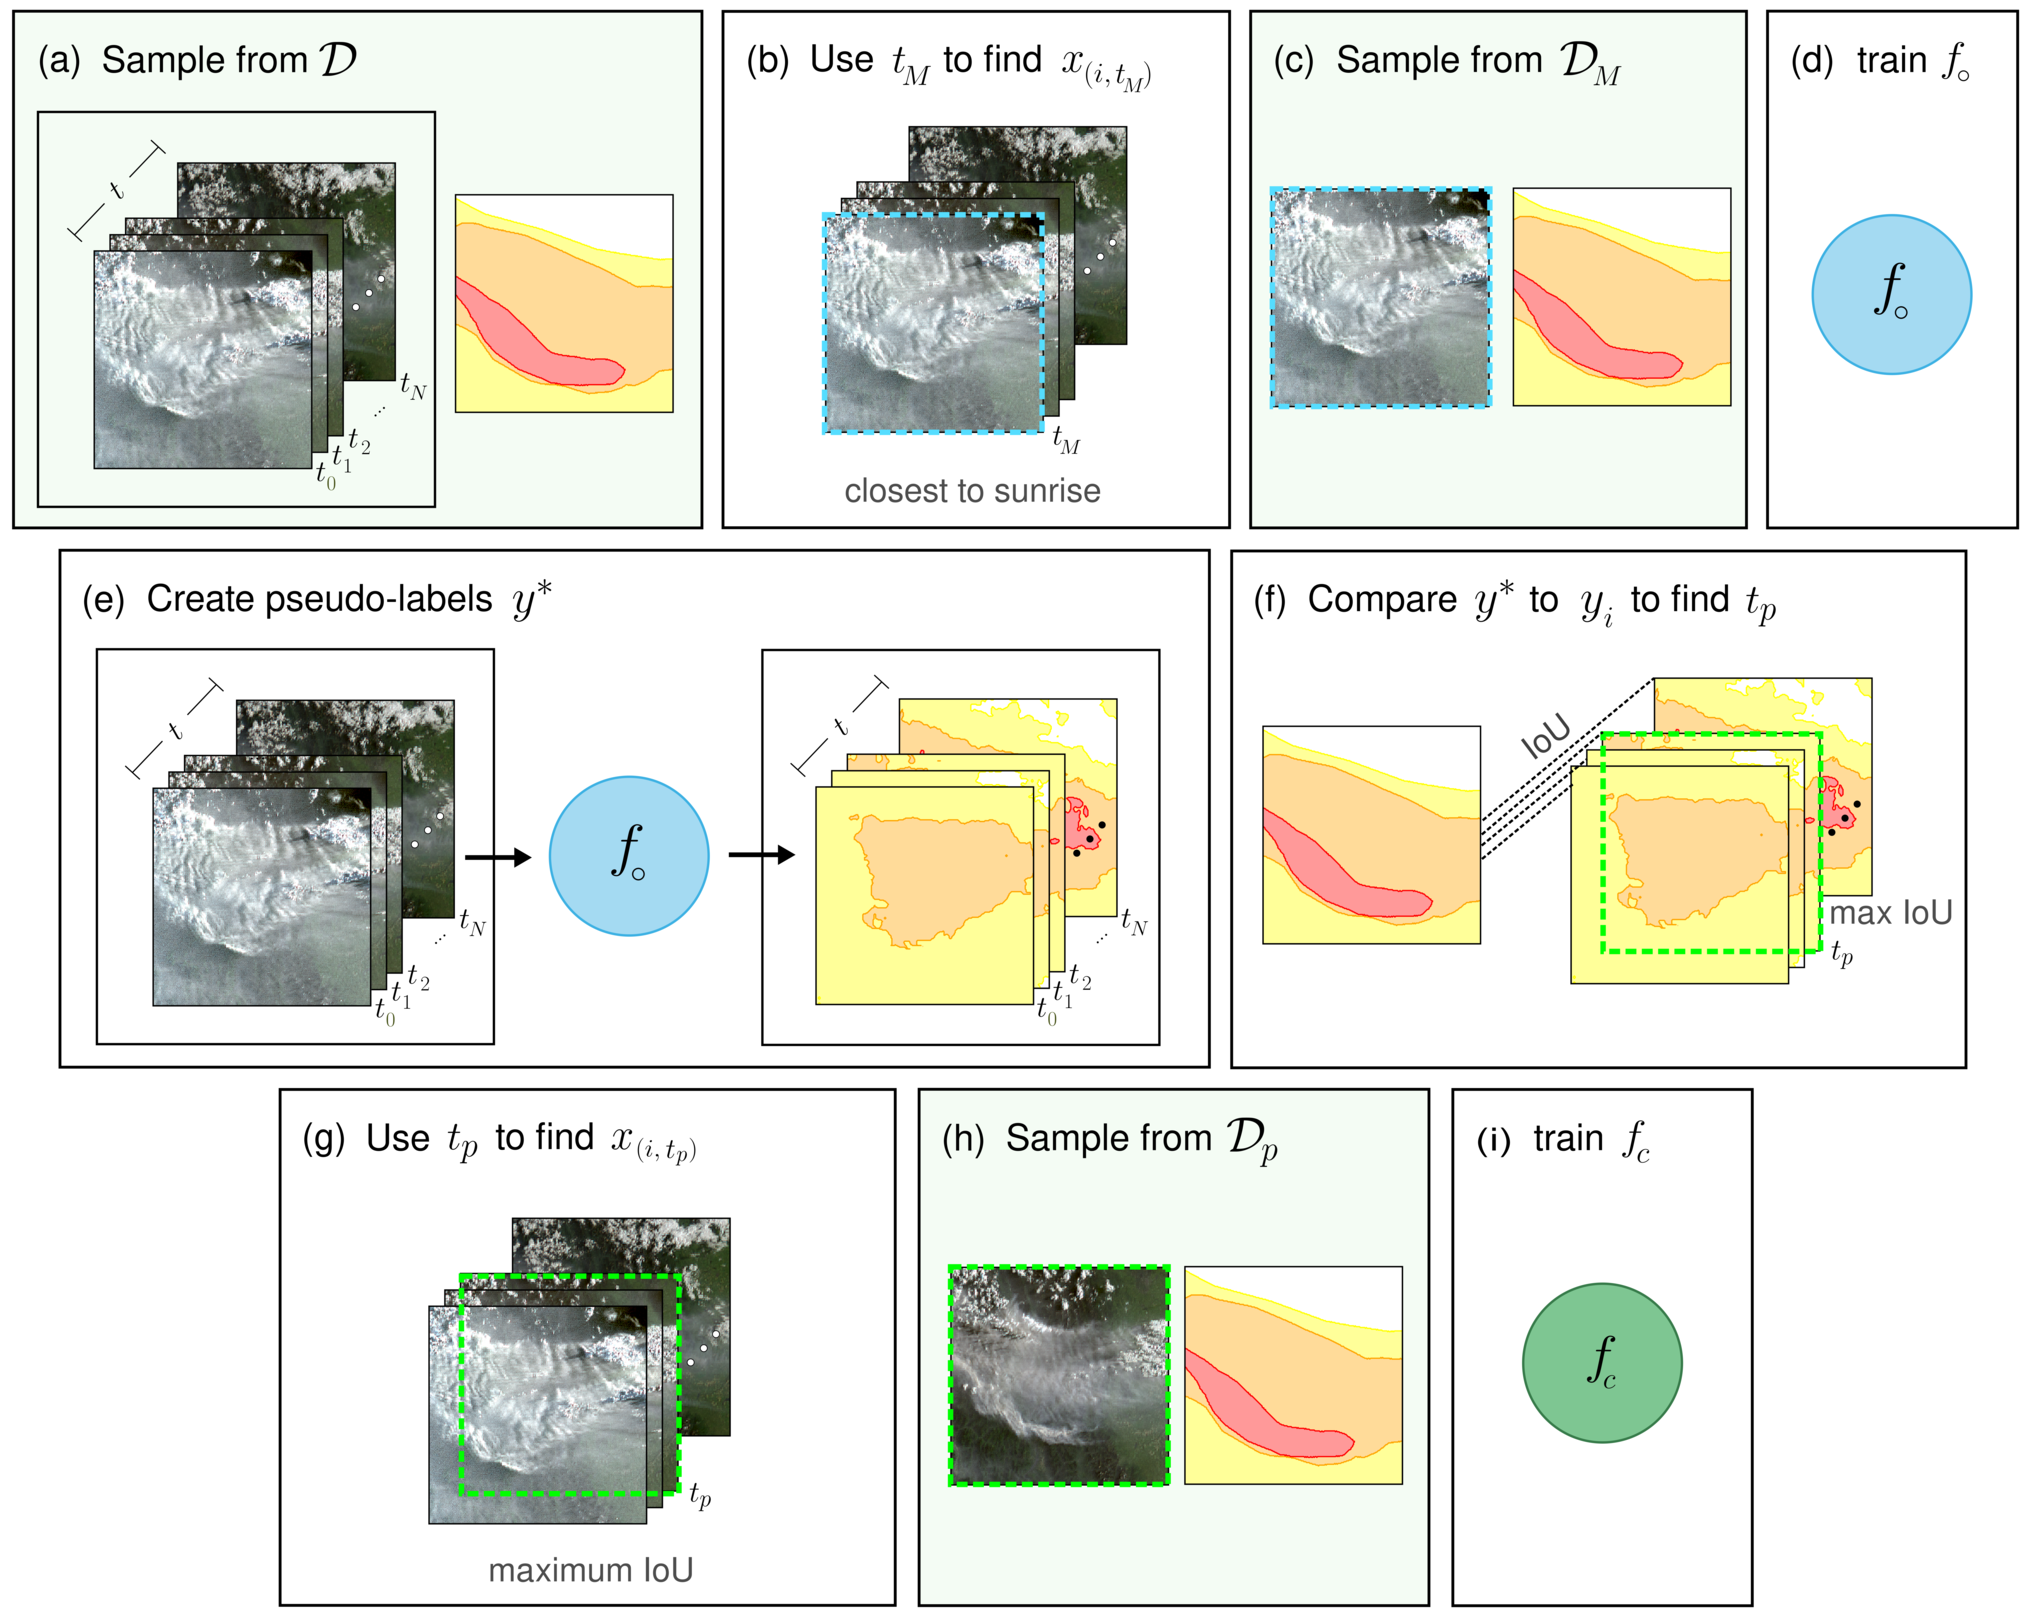
\includegraphics[width=\linewidth]{figures/workflow_small.png}
    \caption{
        PLDR applied to create the SmokeViz dataset. Green boxes indicate dataset stages. 
        (a) For original dataset \(\mathcal{D}\) - analyst annotation \(y_i\) corresponds to \(N\) satellite images across time window \(t\) so that \(([x_{(i,t_0)},...,x_{(i,t_N)}], y_i) \in \mathcal{D}\); 
        (b) use Mie scattering to find the time, \(t_M\), that corresponds with satellite image \(x_{(i,t_M)}\) that would produce the highest possible SNR if smoke was present; 
        (c) resulting \(\mathcal{D}_M\) is one-to-one \((x_{(i,t_M)}, y_i) \in \mathcal{D}_M\);
        (d) parent model \(f_\circ\) is trained on \(\mathcal{D}_M\) such that \(f_\circ(x_{(i,t_M)})=y_i\);
        (e) apply a greedy algorithm \(f_\circ([x_{(i,t_0)},...,x_{(i,t_N)}])=[y^*_{(i,t_0)},...,y^*_{(i,t_N)}]\) to create IPLs \(y^*\) for each candidate image; 
        (f) compute the intersection over union (IoU) between \(y^*\) and \(y_i\) to identify the time \(t_p\) where the IPL and analyst annotation have the maximum IoU; 
        (g) match \(t_p\) to its correpsonding image \(x_{(i,t_p)}\) that is predicted to best match the analyst annotation;
        (h) SmokeViz dataset \(\mathcal{D}_p\) created; 
        (i) child model \(f_c\) is trained on \(\mathcal{D}_p\) such that \(f_c(x_{(i,t_p)})=y_i\) is used to detect and classify the density of wildfire smoke plumes in GOES imagery.
    }
\label{PLDR}
\end{figure}



\begin{table}[!htb]
\parbox{.45\linewidth}{
\centering
    \caption{A comparison of how smoke density would be represented by one-hot encoding commonly used for categorical data to thermometer encoding often used for ordinal data.}\label{therm}
    \begin{tabular}{ccccrrcrc}
        \toprule
        density & one-hot & thermometer \\
        \midrule
        none & \texttt{[0 0 0]} & \texttt{[0 0 0]} \\
        light  & \texttt{[0 0 1]} & \texttt{[0 0 1]} \\
        medium & \texttt{[0 1 0]} & \texttt{[0 1 1]} \\
        heavy  & \texttt{[1 0 0]} & \texttt{[1 1 1]} \\
        \bottomrule
    \end{tabular}
}
\hspace{.4cm}
\parbox{.5\linewidth}{
    \caption{Dataset split for \(\mathcal{D}_M\) and \(\mathcal{D}_p\), samples for 2024 go up to November 1st. We use an entire year of data for both validation and testing sets to capture year-long wildfire trends.}\label{split}
    \centering
    \begin{tabular}{ccccrrcrc}
        \toprule
        dataset & \(\mathcal{D}_M\) & \(\mathcal{D}_p\) &years\\
        \midrule
        training & 165,609 & 144,225 &2018-21, 24\\
        validation & 20,056 & 19,223 &2023 \\
        testing & 21,541 & 20,224 & 2022 \\
        \bottomrule
    \end{tabular}
}
\end{table}

To build \(f_{\circ}\), we implement \texttt{Segmentation Models PyTorch} \cite{semantic} with EfficientNetV2 \cite{efficientnetv2} as the encoder and PSPNet \cite{pspnet} as the decoder. Input images are 256\(\times\)256\(\times\)3 true-color snapshots; the output is a 256\(\times\)256\(\times\)3 classification map predicting categorical smoke density. We use thermometer encoding (Table \ref{therm}) and apply binary cross-entropy loss across density levels. Thermometer encoding is chosen over one-hot encoding because it captures the ordinal structure of smoke density categories (none < light < medium < heavy). In thermometer encoding, each higher class includes all lower class activations (e.g., heavy = [1 1 1]), allowing the model to learn not just class distinctions, but the relative severity of smoke. We use a confidence threshold of IoU  >0.01 \cite{conf_thresh} to exclude samples with negligible overlap. 

\subsection{Benchmark Models}

We benchmark the SmokeViz dataset \(\mathcal{D}_{p}\) using DeepLabV3+ \cite{deeplab} and PSPNet \cite{pspnet} with EfficientNetV2 \cite{efficientnetv2}, DPT \cite{dpt} with ViT \cite{vit}, Segfomer \cite{segformer} and UperNet \cite{upernet} with EfficientVit \cite{efficientvit}. Each model is trained for 100 epochs using a batch size of 16 and the Adam optimizer on 8 16GB Nvidia P100 GPUs. These architectures are selected for their relatively low memory requirements and effectiveness in segmenting multi-scale objects such as smoke plumes.

\section{Results}

We evaluate the performance of \(f_{\circ}\) and \(f_c\) using Intersection over Union (IoU) metrics on the test sets of both \(\mathcal{D}_M\) and \(\mathcal{D}_p\), as shown in Table \ref{iou_results}. For each smoke density class, IoU is calculated as the pixel-level intersection between model predictions and HMS analyst labels, divided by their union, aggregated over all test samples. Overall IoU is computed by summing intersections across all density classes and dividing by the total union of predicted and labeled smoke pixels.

\begin{table}[!htb]
    \caption{IoU results per smoke density and overall, comparing \(f_{\circ}\) and \(f_c\) run on \(\mathcal{D}_M\) and \(\mathcal{D}_p\) test sets.}
    \label{iou_results}
    \centering
    \begin{tabular}{lcc|cc}
        \toprule
        \multicolumn{1}{c}{} & \multicolumn{2}{c}{\(f_{\circ}\)} & \multicolumn{2}{c}{\(f_c\)}\\
        \midrule
        \multicolumn{1}{c}{} & \(\mathcal{D}_M\) & \(\mathcal{D}_{p}\) & \(\mathcal{D}_M\) & \(\mathcal{D}_{p}\) \\
        \midrule
        heavy   & 0.278 & 0.368 & 0.218 &  0.411 \\
        medium  & 0.310 & 0.417 & 0.319 &  0.484 \\
        light   & 0.480 & 0.585 & 0.491 &  0.660 \\
        overall & 0.430 & 0.533 & 0.438 &  0.607 \\
        \bottomrule
    \end{tabular}
\end{table}

\begin{figure}[!htb] 
    \centering
    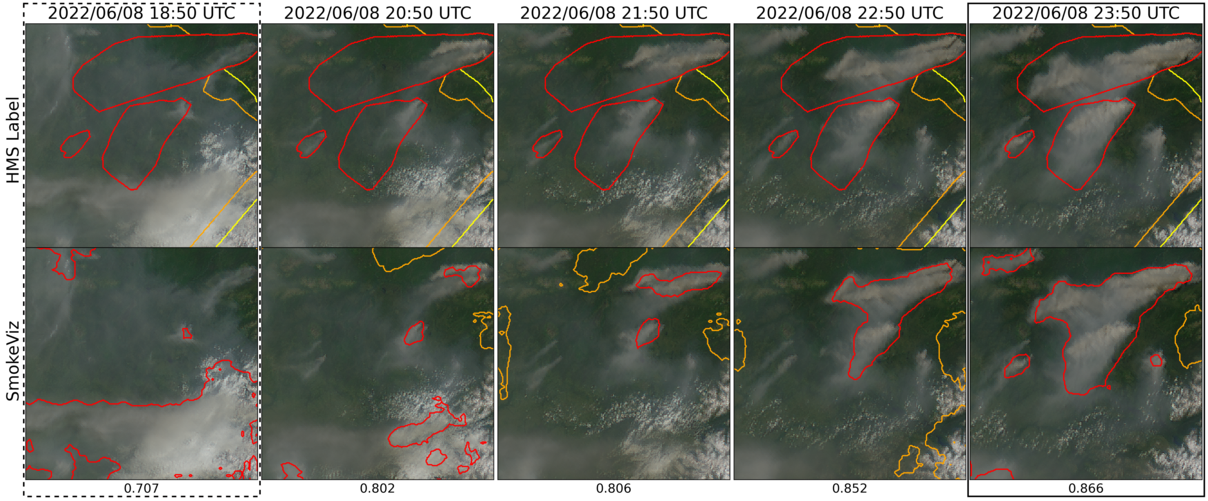
\includegraphics[width=\linewidth]{figures/final_results_small.png}
        \caption{GOES-West imagery from June 8, 2022, over Alaska (\(61.06^{\circ}\)N, \(156.12^{\circ}\)W). Daylight spanned 12:43-7:53 UTC. The HMS annotations (top row) span 18:50-23:50 UTC and are compared with \(f_{\circ}\)-generated smoke predictions (bottom row). The leftmost frame (dotted) represents the Mie-derived image; the rightmost frame (solid) was selected via PLDR and achieves higher IoU.}

    \label{ml_vs_mei}
\end{figure}

Figure \ref{ml_vs_mei} illustrates a case in which the PLDR-selected frame better represents the HMS annotation than the Mie-derived selection. Here, the heavy smoke IoU improves from 0.01 to 0.59. While the Mie-derived image is selected based on its proximity to sunrise, PLDR chooses the frame with the highest overlap between the model-generated intermediary pseudo-label and the analyst annotation. This example highlights PLDR’s advantage in resolving temporal ambiguity.

To further examine the performance of \(f_c\), we can qualitatively compare its predictions against HMS annotations for samples from \(\mathcal{D}_p\) in Figure \ref{examples}. The model outputs capture more spatially detailed and coherent smoke boundaries compared to the coarser, polygon-based analyst labels.

\begin{table}[!htb] 
    \caption{Comparison of segmentation benchmark model IoU metrics on \(\mathcal{D}_{p}\).}\label{bench}
    \centering
    \begin{tabular}{lccccc}
        \toprule
        \textbf{encoder} & EfficientNetV2 \cite{efficientnetv2} & \cite{efficientnetv2} & ViT \cite{vit} & EfficientViT \cite{efficientvit} & \cite{efficientvit}\\
        \textbf{decoder} & DeepLabV3+ \cite{deeplab} & PSPNet \cite{pspnet} & DPT \cite{dpt} & Segformer \cite{segformer} & UperNet \cite{upernet}\\
        \midrule
%        dataset & \multicolumn{5}{c}{\(\mathcal{D}_M\)} \\
%        \midrule
        heavy   & 0.2894 & 0.3222 & 0.2091 & 0.2185 & 0.3099 \\
        medium  & 0.4091 & 0.4289 & 0.3946 & 0.3978 & 0.4042 \\
        light   & 0.4424 & 0.5045 & 0.5155 & 0.4331 & 0.4275 \\
        overall & 0.4172 & 0.4677 & 0.4608 & 0.4055 & 0.4098 \\
        \bottomrule
    \end{tabular}
\end{table}

To benchmark performance across segmentation architectures, we evaluate several encoder-decoder models trained on \(\mathcal{D}_p\). Table \ref{bench} reports IoU scores by smoke density and overall. While DeepLabV3+ achieves the highest IoU for heavy smoke, PSPNet yields the best overall performance. Results across models are relatively consistent, highlighting the robustness of the SmokeViz dataset for training diverse architectures.

\begin{figure}[!htb]
    \centering
    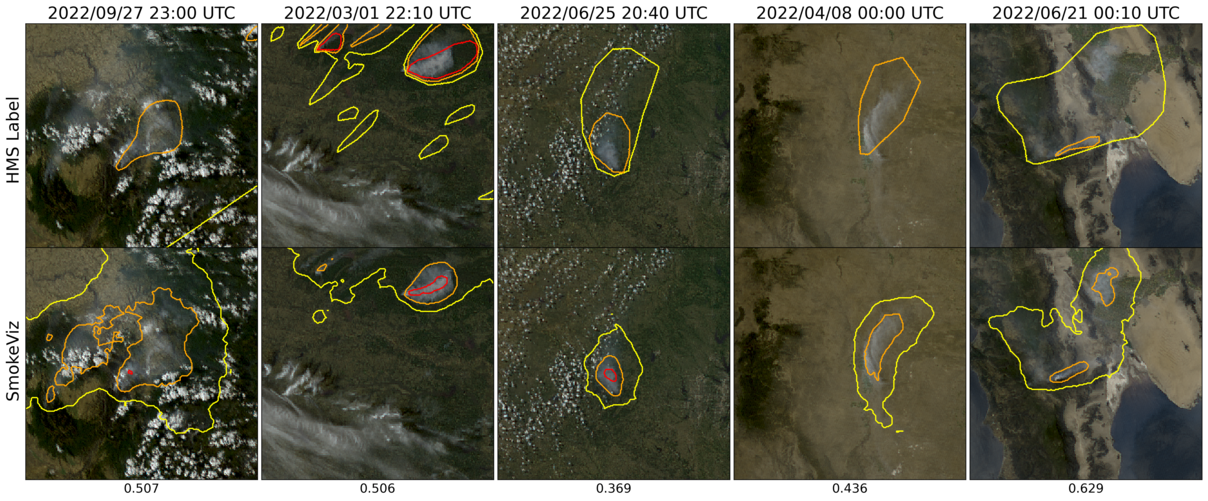
\includegraphics[width=\linewidth]{figures/examples_small.png}
    \caption{Examples of HMS annotations (top row) vs \(f_{c}\) output (bottom row) on \(\mathcal{D}_{p}\) samples. The overall IoU score is reported at the bottom of each column.}\label{examples}
\end{figure}

\section{Limitations}

More discussion and analysis on the two primary limitations can be found in the Supplementary Materials. First, pseudo-labeling methods may propagate biases from the parent model into downstream models. In our case, the increased detectability of forward-scattered light from smoke particulates may bias the model toward higher performance at larger solar zenith angles. Second, the HMS annotations do not distinguish between fire types and include a large number of controlled agricultural burns, which may limit the dataset’s applicability for targeting large-scale wildfires.

Several additional limitations remain important directions for future work. One is evaluating the model’s ability to distinguish smoke from dust. Another is to investigate uncertainty in the analyst annotations. Finally, while we limit the dataset to true-color GOES imagery (bands C01–C03) due to signal-to-noise and dataset size considerations, future studies should investigate the benefits of incorporating additional spectral bands, especially C07. 

\section{Conclusion}

In this study, we present \textbf{SmokeViz}, a refined satellite imagery dataset for semantic segmentation of wildfire smoke plumes. Starting from the original NOAA HMS annotations—coarse, many-to-one approximations of smoke boundaries, we transform the dataset into a one-to-one mapping between satellite frames and smoke annotations. While the Mie-derived dataset selection process maximized the potential for detecting smoke if present, it did not account for whether smoke was actually visible in the selected image, leading to a high incidence of label-image mismatch and associated training noise. To address this, we introduce \textbf{pseudo-label dimension reduction (PLDR)}, a physics-guided, semi-supervised method that uses a parent model trained on the Mie-derived dataset (\(\mathcal{D}_M\)) to generate pseudo-labels across each annotation’s time window. We then select the image with the highest spatial overlap between the intermediary pseudo-label and the HMS annotation to construct a refined dataset (\(\mathcal{D}_p\)). A child model trained on \(\mathcal{D}_p\) achieves higher segmentation performance than the original parent model, as measured by IoU on both test sets, demonstrating the value of pseudo-label-based temporal alignment.


SmokeViz serves as a robust and representative dataset for training models to detect wildfire smoke in GOES imagery at the frame level. In addition to supporting real-time smoke segmentation, this dataset has potential applications in early wildfire detection, air quality monitoring, and as a smoke analysis product for data assimilation into dispersion models. It also provides a challenging benchmark for remote sensing models tasked with segmenting diffuse, low-contrast features like smoke. More generally, this work illustrates how PLDR can be used to resolve resolution mismatches between data and labels, especially in settings with time-series or video data paired with coarse annotations. The dataset is publicly available at \url{https://noaa-gsl-experimental-pds.s3.amazonaws.com/index.html#SmokeViz/} with code available at \url{https://github.com/anonymous-smokeviz/SmokeViz}. 




\bibliography{references}

\end{document}
